\documentclass[11pt,a4paper]{article}
\usepackage[margin=1.7cm]{geometry}
\usepackage[T1]{fontenc}
\usepackage{lmodern}
\usepackage{amsmath,amssymb,mathtools}
\usepackage{booktabs,array,tabularx,longtable,multirow}
\usepackage{xcolor}
\usepackage[most]{tcolorbox}
\usepackage{tikz}
\usetikzlibrary{arrows.meta,positioning,trees,calc,shapes.geometric}
\usepackage{enumitem}
\usepackage{listings}
\usepackage{fancyhdr}
\usepackage{microtype}
\usepackage{hyperref}
\usepackage{graphicx}

\definecolor{primary}{HTML}{1E4F91}
\definecolor{qblue}{HTML}{2F80ED}
\definecolor{qback}{HTML}{EEF6FF}
\definecolor{agreen}{HTML}{239653}
\definecolor{aback}{HTML}{EFFAF2}
\definecolor{warn}{HTML}{D97706}
\definecolor{softgray}{HTML}{F4F6F8}
\definecolor{deepnavy}{HTML}{17324D}
\definecolor{redsoft}{HTML}{FFF1F1}

\hypersetup{colorlinks=true,linkcolor=primary,urlcolor=primary}
\pagestyle{fancy}
\fancyhf{}
\lhead{CSE-3203: Design and Analysis of Algorithms - II}
\rhead{Final 2023 - Complete Q\&A}
\cfoot{\thepage}
\setlength{\headheight}{14pt}
\setlength{\parindent}{0pt}
\setlength{\parskip}{4pt}

\newtcolorbox{qaquestion}[1][]{
  enhanced,breakable,
  colback=qback,colframe=qblue,
  coltitle=white,fonttitle=\bfseries,
  title=#1,
  boxrule=0.9pt,arc=2mm,
  left=3mm,right=3mm,top=2mm,bottom=2mm,
  before skip=8pt,after skip=5pt
}
\newtcolorbox{qaanswer}[1][]{
  enhanced,breakable,
  colback=aback,colframe=agreen,
  coltitle=white,fonttitle=\bfseries,
  title=#1,
  boxrule=0.9pt,arc=2mm,
  left=3mm,right=3mm,top=2mm,bottom=2mm,
  before skip=2pt,after skip=10pt
}
\newtcolorbox{pointbox}[1][]{
  enhanced,breakable,colback=softgray,colframe=deepnavy,
  title=#1,fonttitle=\bfseries,coltitle=white,
  boxrule=.8pt,arc=1.5mm
}
\newtcolorbox{warningbox}[1][]{
  enhanced,breakable,colback=redsoft,colframe=warn,
  title=#1,fonttitle=\bfseries,coltitle=white,
  boxrule=.8pt,arc=1.5mm
}

\lstset{
  basicstyle=\ttfamily\small,
  frame=single,
  backgroundcolor=\color{white},
  rulecolor=\color{deepnavy!50},
  columns=fullflexible,
  keepspaces=true,
  showstringspaces=false,
  breaklines=true
}

\newcommand{\Oh}{\mathcal{O}}
\newcommand{\OPT}{\mathrm{OPT}}
\newcommand{\UB}{\mathrm{UB}}
\newcommand{\LB}{\mathrm{LB}}

\begin{document}

\begin{center}
{\Huge\bfseries\color{primary} CSE-3203 Final Examination 2023}\\[0.25em]
{\Large\color{deepnavy} Complete Questions and Answers}\\[0.35em]
{\normalsize Design and Analysis of Algorithms - II}
\end{center}

\begin{pointbox}[How to use these notes]
The questions are transcribed from the two supplied exam-page screenshots and answered in an exam-ready form. For the slightly blurred KMP text in Question 4(b), the scan is read as \(P=\texttt{abbaab}\) and \(T=\texttt{abaabbaabbbababa}\); the solution below is based on that reading.
\end{pointbox}

% ==================== Q1 ====================
\begin{qaquestion}[Question 1(a) - 4 marks]
Define primary clustering in context of hashing. Explain the effect of primary clustering and the mechanism to reduce it.
\end{qaquestion}
\begin{qaanswer}[Answer 1(a)]
\textbf{Primary clustering} occurs in open addressing, especially \textbf{linear probing}, when consecutive occupied slots form long blocks (clusters). If a new key hashes anywhere into or just before such a block, linear probing tends to append the new key to that block, making the cluster even larger.

\textbf{Effect.}
\begin{itemize}[leftmargin=*]
\item Long runs of occupied cells are created.
\item Successful and unsuccessful searches require more probes.
\item Insertions become slower as the load factor \(\alpha=n/m\) grows.
\item Clusters attract more keys, so the problem reinforces itself.
\end{itemize}

\textbf{How to reduce it.}
\begin{enumerate}[leftmargin=*]
\item \textbf{Quadratic probing:} use
\[
h(k,i)=\bigl(h'(k)+c_1i+c_2i^2\bigr)\bmod m.
\]
The non-linear jumps break up primary clusters, although keys with the same initial hash may still have \emph{secondary clustering}.
\item \textbf{Double hashing:} use
\[
h(k,i)=\bigl(h_1(k)+i\,h_2(k)\bigr)\bmod m.
\]
Different keys usually get different probe steps, so both primary and much of secondary clustering are reduced.
\item Keep the load factor moderate and resize/rehash when the table becomes too full.
\end{enumerate}

\textbf{Memory line:} Linear probing \(\to\) primary clustering; quadratic probing reduces it; double hashing usually spreads probes best.
\end{qaanswer}

\begin{qaquestion}[Question 1(b) - 6 marks]
Insert the keys
\[
10,22,31,4,15,28,17,88,59
\]
into a hash table of length \(m=11\) using open addressing with \(h'(k)=k\bmod 11\). Illustrate the result using:

(i) quadratic probing with \(c_1=1\) and \(c_2=3\), and

(ii) double hashing with \(h_1(k)=k\bmod 11\) and \(h_2(k)=1+(k\bmod 10)\).
\end{qaquestion}
\begin{qaanswer}[Answer 1(b)]
\textbf{(i) Quadratic probing}
\[
h(k,i)=\bigl(k\bmod 11+i+3i^2\bigr)\bmod 11,\qquad i=0,1,2,\ldots
\]

\begin{center}
\small
\begin{tabular}{c l c}
\toprule
Key & Probe sequence until insertion & Final slot\\
\midrule
10 & 10 & 10\\
22 & 0 & 0\\
31 & 9 & 9\\
4  & 4 & 4\\
15 & 4, 8 & 8\\
28 & 6 & 6\\
17 & 6, 10, 9, 3 & 3\\
88 & 0, 4, 3, 8, 8, 3, 4, 0, 2 & 2\\
59 & 4, 8, 7 & 7\\
\bottomrule
\end{tabular}
\end{center}

The repeated locations in the probe sequence for 88 occur because the given quadratic constants do not generate a new slot at every value of \(i\).

\begin{center}
\begin{tabular}{c|ccccccccccc}
Index &0&1&2&3&4&5&6&7&8&9&10\\\hline
Value &22&--&88&17&4&--&28&59&15&31&10
\end{tabular}
\end{center}

\textbf{(ii) Double hashing}
\[
h(k,i)=\bigl(h_1(k)+i h_2(k)\bigr)\bmod 11,
\]
where
\[
h_1(k)=k\bmod 11,\qquad h_2(k)=1+(k\bmod 10).
\]

\begin{center}
\small
\begin{tabular}{c l c}
\toprule
Key & Probe sequence until insertion & Final slot\\
\midrule
10 & 10 & 10\\
22 & 0 & 0\\
31 & 9 & 9\\
4  & 4 & 4\\
15 & 4, 10, 5 & 5\\
28 & 6 & 6\\
17 & 6, 3 & 3\\
88 & 0, 9, 7 & 7\\
59 & 4, 3, 2 & 2\\
\bottomrule
\end{tabular}
\end{center}

\begin{center}
\begin{tabular}{c|ccccccccccc}
Index &0&1&2&3&4&5&6&7&8&9&10\\\hline
Value &22&--&59&17&4&15&28&88&--&31&10
\end{tabular}
\end{center}

Double hashing produces a much more varied probe sequence and avoids the long repeated pattern seen in the quadratic case.
\end{qaanswer}

\begin{qaquestion}[Question 1(c) - 4 marks]
Prove that the expected number of probes in an unsuccessful search is at most
\[
\frac{1}{1-\alpha}
\]
for an open-address hash table with load factor \(\alpha=n/m<1\), assuming uniform hashing.
\end{qaquestion}
\begin{qaanswer}[Answer 1(c)]
Let \(X\) be the number of probes performed in an unsuccessful search. Under uniform hashing, the probability that the first probed location is occupied is \(n/m=\alpha\).

The probability that the first \(i\) probed positions are all occupied is
\[
\frac{n}{m}\cdot\frac{n-1}{m-1}\cdots
\frac{n-i+1}{m-i+1}
\le \left(\frac{n}{m}\right)^i
=\alpha^i.
\]
Hence
\[
\Pr(X>i)\le \alpha^i.
\]
Using the tail-sum formula for a positive integer-valued random variable,
\[
\mathbb E[X]
=\sum_{i\ge0}\Pr(X>i)
\le \sum_{i\ge0}\alpha^i.
\]
Since \(0\le\alpha<1\), the geometric series gives
\[
\boxed{\mathbb E[X]\le \frac{1}{1-\alpha}}.
\]
Thus, for example, at \(\alpha=0.5\) the expected unsuccessful-search cost is at most 2 probes.
\end{qaanswer}

% ==================== Q2 ====================
\begin{qaquestion}[Question 2(a) - 3 marks]
Define the state-space tree. Describe the features of a node of a state-space tree in the context of backtracking.
\end{qaquestion}
\begin{qaanswer}[Answer 2(a)]
A \textbf{state-space tree} is a rooted tree that represents all candidate states/partial solutions that can be generated while solving a combinatorial problem.

\textbf{Node features in backtracking:}
\begin{itemize}[leftmargin=*]
\item \textbf{Root:} empty or initial solution.
\item \textbf{Level:} the number of decisions already made.
\item \textbf{State/partial solution:} choices made from the root to that node.
\item \textbf{Children:} possible next choices.
\item \textbf{Promising node:} may still lead to a feasible/optimal solution, so it is expanded.
\item \textbf{Non-promising node:} violates a constraint or cannot lead to a solution, so it is pruned.
\item \textbf{Solution leaf:} a complete feasible solution.
\end{itemize}
Backtracking performs a depth-first exploration and returns to an earlier node whenever the current node becomes non-promising.
\end{qaanswer}

\begin{qaquestion}[Question 2(b) - 5 marks]
Design a linear-time algorithm that finds a solution to the \(n\)-queens problem for any \(n\ge4\).
\end{qaquestion}
\begin{qaanswer}[Answer 2(b)]
A constructive \(\Oh(n)\) method outputs the column positions of the queens directly. Let
\[
E=(2,4,6,\ldots),\qquad O=(1,3,5,\ldots)
\]
be the even and odd column lists up to \(n\). The \(i\)-th output number is the column of the queen in row \(i\).

\begin{enumerate}[leftmargin=*]
\item If \(n\bmod 6\notin\{2,3\}\), output \(E\) followed by \(O\).
\item If \(n\bmod6=2\), output \(E\), then in \(O\) swap 1 and 3 and move 5 to the end.
\item If \(n\bmod6=3\), move 2 to the end of \(E\); move 1 and 3 to the end of \(O\); then output \(E\) followed by \(O\).
\end{enumerate}

\textbf{Examples}
\[
n=8:\quad [2,4,6,8,3,1,7,5],
\]
\[
n=9:\quad [4,6,8,2,5,7,9,1,3].
\]
Each list contains every column exactly once, and the construction avoids equal diagonal differences. Creating and printing the two lists takes \(\boxed{\Oh(n)}\) time.
\end{qaanswer}

\begin{qaquestion}[Question 2(c) - 6 marks]
Apply backtracking to find a Hamiltonian circuit in the given graph.
\end{qaquestion}
\begin{qaanswer}[Answer 2(c)]
One successful backtracking path is
\[
\boxed{c\to a\to b\to e\to g\to d\to f\to c}.
\]
It visits every vertex \(\{a,b,c,d,e,f,g\}\) exactly once and returns to the start.

\begin{center}
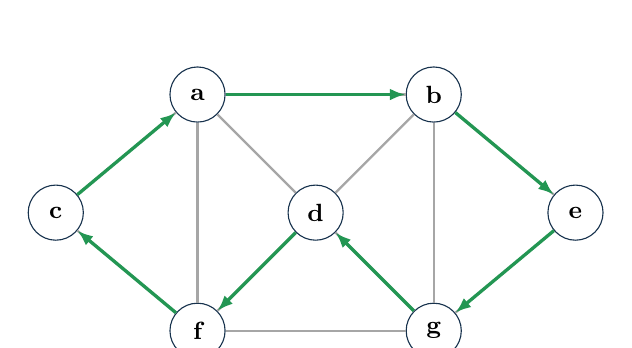
\begin{tikzpicture}[
  v/.style={circle,draw=deepnavy,fill=white,minimum size=7mm,font=\small\bfseries},
  e/.style={draw=gray!70,thick},
  h/.style={draw=agreen,very thick,-{Latex[length=2mm]}}
]
\node[v] (a) at (0,2) {a};
\node[v] (b) at (3,2) {b};
\node[v] (c) at (-1.8,0.5) {c};
\node[v] (d) at (1.5,0.5) {d};
\node[v] (e1) at (4.8,0.5) {e};
\node[v] (f) at (0,-1) {f};
\node[v] (g) at (3,-1) {g};
\foreach \x/\y in {a/b,a/c,c/f,a/f,a/d,f/d,d/b,d/g,f/g,b/g,b/e1,g/e1} \draw[e] (\x)--(\y);
\draw[h] (c)--(a);
\draw[h] (a)--(b);
\draw[h] (b)--(e1);
\draw[h] (e1)--(g);
\draw[h] (g)--(d);
\draw[h] (d)--(f);
\draw[h] (f)--(c);
\end{tikzpicture}
\end{center}

\textbf{Backtracking idea.} Start at \(c\). Add an adjacent unvisited vertex. If a partial path has no unused adjacent vertex that can eventually return to \(c\), undo the last choice and try another neighbor. The path above completes successfully, so search can stop if only one Hamiltonian circuit is required.
\end{qaanswer}

% ==================== Q3 ====================
\begin{qaquestion}[Question 3(a) - 4 marks]
Describe the best-first branch-and-bound approach with a suitable example.
\end{qaquestion}
\begin{qaanswer}[Answer 3(a)]
In \textbf{best-first branch and bound}, all live nodes are kept in a priority queue. The algorithm always expands the live node with the most promising bound.

\textbf{For maximization:}
\[
\text{choose largest upper bound (UB)},\qquad
\UB\le \text{bestValue}\Rightarrow\text{prune}.
\]

\textbf{For minimization:}
\[
\text{choose smallest lower bound (LB)},\qquad
\LB\ge \text{bestValue}\Rightarrow\text{prune}.
\]

\textbf{Small maximization example.} Suppose live nodes have upper bounds 92, 75 and 88 while the best feasible solution found so far has value 80. Best-first expands the node with UB 92 first; the node with UB 75 is immediately pruned because it cannot beat 80. A priority queue makes the next-node selection efficient.

\textbf{General steps:}
\begin{enumerate}[leftmargin=*]
\item Create the root and compute its bound.
\item Remove the best-bound live node from the priority queue.
\item Branch into children.
\item Reject infeasible children.
\item Update the incumbent (best complete feasible solution).
\item Insert only children whose bound can still improve the incumbent.
\item Repeat until no live node remains.
\end{enumerate}
\end{qaanswer}

\begin{qaquestion}[Question 3(b) - 2 marks]
Give an example of a best-case input for an assignment problem in the context of branch and bound.
\end{qaquestion}
\begin{qaanswer}[Answer 3(b)]
For a minimization assignment problem, a best-case input is one where the optimal assignment is immediately obvious and every alternative branch gets a much larger lower bound. For example,
\[
C=\begin{bmatrix}
0&100&100\\
100&0&100\\
100&100&0
\end{bmatrix}.
\]
The diagonal assignment \((1\to1,2\to2,3\to3)\) has cost 0. Once this complete solution is found, every branch containing any off-diagonal assignment has lower bound at least 100, so all such branches are pruned immediately. Hence very few nodes are expanded.
\end{qaanswer}

\begin{qaquestion}[Question 3(c) - 8 marks]
Solve the following 0/1 knapsack problem using branch and bound.

\begin{center}
\begin{tabular}{c c c}
\toprule
Item & Weight & Value (BDT)\\
\midrule
1&10&100\\
2&7&63\\
3&8&56\\
4&4&12\\
\bottomrule
\end{tabular}
\qquad Capacity \(W=16\).
\end{center}
\end{qaquestion}
\begin{qaanswer}[Answer 3(c)]
First sort by value/weight ratio:
\[
\frac{100}{10}=10,\quad \frac{63}{7}=9,\quad \frac{56}{8}=7,\quad \frac{12}{4}=3.
\]
The items are already in decreasing ratio order. Use the fractional-knapsack value as an upper bound.

\textbf{Root bound:}
\[
100+6\left(\frac{63}{7}\right)=100+54=154.
\]

The important best-first search nodes are:
\begin{center}
\small
\begin{tabular}{c c c c l}
\toprule
Decision path & Weight & Profit & UB & Action\\
\midrule
root &0&0&154&expand\\
1 &10&100&154&expand\\
11 &17&163&--&infeasible\\
10 &10&100&142&live\\
0 &0&0&122&live\\
101 &18&156&--&infeasible\\
100 &10&100&112&later prune\\
01 &7&63&122&expand\\
00 &0&0&68&prune\\
011 &15&119&122&expand\\
010 &7&63&75&prune\\
0111 &19&131&--&infeasible\\
0110 &15&119&119&complete solution\\
\bottomrule
\end{tabular}
\end{center}
Here 1 means ``take the current item'' and 0 means ``skip it.''

\begin{center}
\resizebox{0.96\textwidth}{!}{%
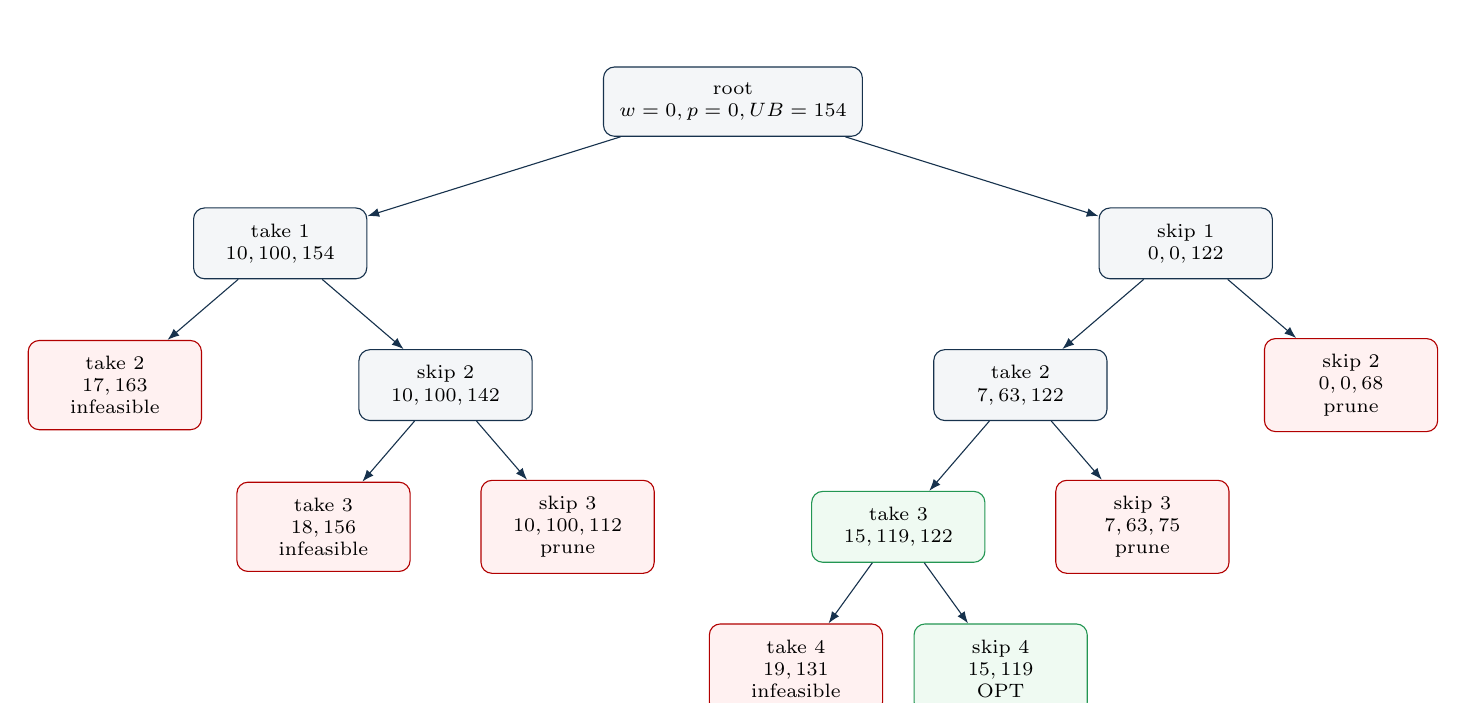
\begin{tikzpicture}[
 level distance=18mm,
 level 1/.style={sibling distance=115mm},
 level 2/.style={sibling distance=42mm},
 level 3/.style={sibling distance=31mm},
 level 4/.style={sibling distance=26mm},
 n/.style={draw=deepnavy,rounded corners,fill=softgray,align=center,font=\scriptsize,inner sep=2mm,minimum width=22mm},
 good/.style={draw=agreen,rounded corners,fill=aback,align=center,font=\scriptsize,inner sep=2mm,minimum width=22mm},
 bad/.style={draw=red!70!black,rounded corners,fill=redsoft,align=center,font=\scriptsize,inner sep=2mm,minimum width=22mm},
 edge from parent/.style={draw=deepnavy,-{Latex[length=1.5mm]}}
]
\node[n]{root\\\(w=0,p=0,UB=154\)}
 child {node[n]{take 1\\\(10,100,154\)}
   child {node[bad]{take 2\\\(17,163\)\\infeasible}}
   child {node[n]{skip 2\\\(10,100,142\)}
     child {node[bad]{take 3\\\(18,156\)\\infeasible}}
     child {node[bad]{skip 3\\\(10,100,112\)\\prune}}
   }
 }
 child {node[n]{skip 1\\\(0,0,122\)}
   child {node[n]{take 2\\\(7,63,122\)}
     child {node[good]{take 3\\\(15,119,122\)}
       child {node[bad]{take 4\\\(19,131\)\\infeasible}}
       child {node[good]{skip 4\\\(15,119\)\\OPT}}
     }
     child {node[bad]{skip 3\\\(7,63,75\)\\prune}}
   }
   child {node[bad]{skip 2\\\(0,0,68\)\\prune}}
 };
\end{tikzpicture}%
}
\end{center}

After finding profit 119, every remaining live node has \(UB\le119\) (in particular the node with UB 112), so it is pruned.

Therefore the optimal choice is
\[
\boxed{\{\text{item 2, item 3}\}},\qquad
\boxed{\text{weight}=7+8=15},\qquad
\boxed{\text{maximum value}=63+56=\text{BDT }119}.
\]
\end{qaanswer}

% ==================== Q4 ====================
\begin{qaquestion}[Question 4(a) - 4 marks]
Write any string-matching algorithm that, given a pattern \(P\), finds its occurrences in a text \(T\). Analyze the complexity of the written algorithm in detail.
\end{qaquestion}
\begin{qaanswer}[Answer 4(a)]
A suitable answer is the \textbf{Knuth-Morris-Pratt (KMP)} algorithm.

Let \(m=|P|\), \(n=|T|\), and let \(\pi[q]\) be the length of the longest proper prefix of \(P[0..q]\) that is also a suffix.

\begin{lstlisting}
KMP-MATCH(T, P)
    pi = PREFIX-FUNCTION(P)
    q = 0
    for i = 0 to n-1
        while q > 0 and P[q] != T[i]
            q = pi[q-1]
        if P[q] == T[i]
            q = q + 1
        if q == m
            report occurrence at i-m+1
            q = pi[m-1]
\end{lstlisting}

\textbf{Complexity.}
\begin{itemize}[leftmargin=*]
\item Prefix-function computation: \(\Oh(m)\).
\item Text scan: \(\Oh(n)\). Although the while-loop can execute several times at one position, \(q\) can increase only \(n\) times overall and each fallback decreases it, giving linear amortized work.
\item Total time: \(\boxed{\Oh(n+m)}\).
\item Extra space: \(\boxed{\Oh(m)}\) for the prefix array.
\end{itemize}
KMP never moves the text pointer backward.
\end{qaanswer}

\begin{qaquestion}[Question 4(b) - 6 marks]
You are given a pattern \(P=\texttt{abbaab}\) and a text \(T=\texttt{abaabbaabbbababa}\). Apply the KMP string-matching algorithm to find the occurrences of \(P\) in \(T\). Write the prefix function/array and simulate the solution.
\end{qaquestion}
\begin{qaanswer}[Answer 4(b)]
\textbf{Prefix function for \(P=\texttt{abbaab}\).}

\begin{center}
\begin{tabular}{c|cccccc}
Index \(i\) &0&1&2&3&4&5\\\hline
\(P[i]\)&a&b&b&a&a&b\\
\(\pi[i]\)&0&0&0&1&1&2
\end{tabular}
\end{center}
Thus
\[
\boxed{\pi=[0,0,0,1,1,2]}.
\]

A compact KMP trace is shown below. \(q\) is the number of currently matched pattern characters after processing \(T[i]\); when a full match is found, KMP reports it and resets \(q\) using \(\pi\).

\begin{center}
\small
\begin{tabular}{c c c l}
\toprule
\(i\) & \(T[i]\) & Resulting \(q\) & Note\\
\midrule
0&a&1&match a\\
1&b&2&match ab\\
2&a&1&fallback \(2\to0\), then match a\\
3&a&1&fallback \(1\to0\), then match a\\
4&b&2&match\\
5&b&3&match\\
6&a&4&match\\
7&a&5&match\\
8&b&2&full match \(P\) at start 3; reset \(q=\pi[5]=2\)\\
9&b&3&continue\\
10&b&0&fallback \(3\to0\), mismatch\\
11&a&1&match\\
12&b&2&match\\
13&a&1&fallback \(2\to0\), then match a\\
14&b&2&match\\
15&a&1&fallback \(2\to0\), then match a\\
\bottomrule
\end{tabular}
\end{center}

The occurrence is
\[
T[3..8]=\texttt{abbaab}.
\]
Therefore
\[
\boxed{\text{one occurrence at 0-based shift }3}
\]
or equivalently at the \(\boxed{4\text{th character}}\) in 1-based indexing.
\end{qaanswer}

\begin{qaquestion}[Question 4(c) - 4 marks]
Given \(S=\texttt{caabcba}\), write an algorithm to remove the minimum number of characters so that \(S\) becomes a palindrome. Show the resultant string.
\end{qaquestion}
\begin{qaanswer}[Answer 4(c)]
The minimum-deletion problem is equivalent to finding a \textbf{longest palindromic subsequence (LPS)}.
\[
\boxed{\text{minimum deletions}=n-\mathrm{LPS}(S)}.
\]
A standard dynamic-programming recurrence is
\[
L[i][j]=
\begin{cases}
1, & i=j,\\
2+L[i+1][j-1], & S[i]=S[j],\\
\max(L[i+1][j],L[i][j-1]), & S[i]\ne S[j].
\end{cases}
\]
Fill the table by increasing substring length and reconstruct one LPS by walking backward through the table.

For
\[
S=\texttt{c a a b c b a},\qquad n=7,
\]
one LPS is
\[
\boxed{\texttt{abcba}}
\]
of length 5. Thus
\[
\boxed{7-5=2\text{ deletions}}.
\]
For example, delete the initial \texttt{c} and the second extra \texttt{a}; the resultant string is
\[
\boxed{\texttt{abcba}},
\]
which is a palindrome.

The DP runs in \(\Oh(n^2)\) time and \(\Oh(n^2)\) space (or \(\Oh(n)\) space if only the count is needed).
\end{qaanswer}

% ==================== Q5 ====================
\begin{qaquestion}[Question 5(a) - 7 marks]
Explain the Marker's Algorithm. Apply the algorithm to the following pseudocode to extract the results.
\begin{lstlisting}
1. def func(a, b):
2.     c = a + b
3.     d = 2 * c - a
4.     e = 10
5.     f = 2 * d
6.     print(f)
\end{lstlisting}
\end{qaquestion}
\begin{qaanswer}[Answer 5(a)]
In the context of this pseudocode, \textbf{Marker's Algorithm} is a backward dependence-marking method used to identify statements that contribute to the required output. (This is different from the randomized paging ``marking algorithm.'')

\textbf{Procedure.}
\begin{enumerate}[leftmargin=*]
\item Mark the output/use statement(s).
\item If a marked statement uses a variable, mark the statement that defines that variable.
\item Recursively mark all variables and definitions needed by those marked statements.
\item Any unmarked assignment is irrelevant/dead for the requested output and can be removed.
\end{enumerate}

Apply it backward from \texttt{print(f)}:
\[
\texttt{print(f)}\Rightarrow f\Rightarrow d\Rightarrow(c,a)\Rightarrow(a,b).
\]
So the marked lines are 2, 3, 5 and 6 (plus the function header). Line 4, \texttt{e = 10}, is never used and remains unmarked.

\begin{center}
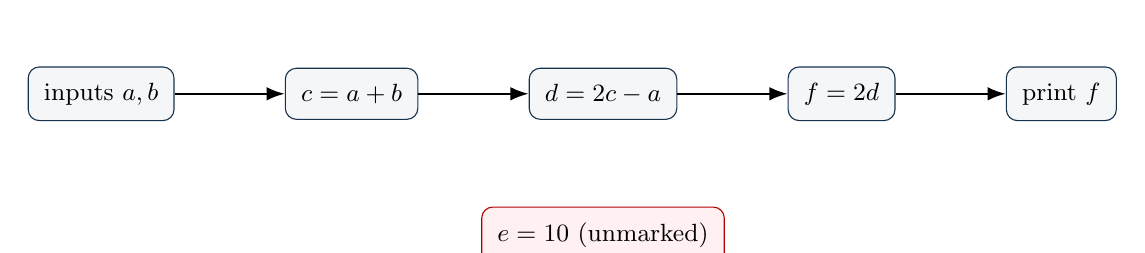
\begin{tikzpicture}[>=Latex,node distance=11mm and 14mm,
 var/.style={draw=deepnavy,rounded corners,fill=softgray,inner sep=2mm,font=\small}]
\node[var] (ab) {inputs \(a,b\)};
\node[var, right=of ab] (c) {\(c=a+b\)};
\node[var, right=of c] (d) {\(d=2c-a\)};
\node[var, right=of d] (f) {\(f=2d\)};
\node[var, right=of f] (o) {print \(f\)};
\draw[->,thick] (ab)--(c);
\draw[->,thick] (c)--(d);
\draw[->,thick] (d)--(f);
\draw[->,thick] (f)--(o);
\node[var, below=of d, draw=red!70!black,fill=redsoft] (e) {\(e=10\) (unmarked)};
\end{tikzpicture}
\end{center}

The extracted/optimized program is
\begin{lstlisting}
def func(a, b):
    c = a + b
    d = 2 * c - a
    f = 2 * d
    print(f)
\end{lstlisting}
Symbolically,
\[
d=2(a+b)-a=a+2b,
\qquad
f=2d=\boxed{2a+4b}.
\]
\end{qaanswer}

\begin{qaquestion}[Question 5(b) - 7 marks]
Solve the system of congruences using the Chinese Remainder Theorem (CRT):
\[
x\equiv2\pmod3,\qquad
x\equiv3\pmod5,\qquad
x\equiv2\pmod7.
\]
Find the smallest positive integer satisfying all three.
\end{qaquestion}
\begin{qaanswer}[Answer 5(b)]
The moduli 3, 5 and 7 are pairwise coprime, so CRT applies.
\[
N=3\cdot5\cdot7=105.
\]
Define
\[
N_1=105/3=35,\quad N_2=105/5=21,\quad N_3=105/7=15.
\]
Find inverses:
\[
35\equiv2\pmod3,\quad 2^{-1}\equiv2\pmod3,
\]
\[
21\equiv1\pmod5,\quad 1^{-1}\equiv1\pmod5,
\]
\[
15\equiv1\pmod7,\quad 1^{-1}\equiv1\pmod7.
\]
Hence
\[
\begin{aligned}
x&\equiv 2(35)(2)+3(21)(1)+2(15)(1)\pmod{105}\\
&=140+63+30\\
&=233\\
&\equiv23\pmod{105}.
\end{aligned}
\]
Therefore the smallest positive solution is
\[
\boxed{x=23}.
\]
Check: \(23\bmod3=2\), \(23\bmod5=3\), \(23\bmod7=2\).
\end{qaanswer}

% ==================== Q6 ====================
\begin{qaquestion}[Question 6(a) - 2 marks]
State the decision version of the Independent Set and Vertex Cover problems.
\end{qaquestion}
\begin{qaanswer}[Answer 6(a)]
\textbf{Independent Set (decision).} Given a graph \(G=(V,E)\) and integer \(k\), does there exist a set \(S\subseteq V\) with \(|S|\ge k\) such that no two vertices in \(S\) are adjacent?

\textbf{Vertex Cover (decision).} Given a graph \(G=(V,E)\) and integer \(k\), does there exist a set \(C\subseteq V\) with \(|C|\le k\) such that every edge in \(E\) has at least one endpoint in \(C\)?
\end{qaanswer}

\begin{qaquestion}[Question 6(b) - 6 marks]
Establish a relationship between Independent Set and Vertex Cover that transforms an input instance of one problem into an input instance of the other. State the relationship as a lemma and prove it.
\end{qaquestion}
\begin{qaanswer}[Answer 6(b)]
\textbf{Lemma.} For any graph \(G=(V,E)\), a set \(S\subseteq V\) is an independent set if and only if \(V-S\) is a vertex cover.

\textbf{Proof (\(\Rightarrow\)).} Suppose \(S\) is independent. No edge can have both endpoints in \(S\). Therefore every edge has at least one endpoint in \(V-S\). Hence \(V-S\) is a vertex cover.

\textbf{Proof (\(\Leftarrow\)).} Suppose \(V-S\) is a vertex cover. If two vertices of \(S\) were adjacent, the edge between them would have neither endpoint in \(V-S\), contradicting that \(V-S\) covers every edge. Hence \(S\) is independent.

Therefore,
\[
\boxed{G\text{ has an independent set of size }k
\iff
G\text{ has a vertex cover of size }|V|-k.}
\]
The reduction simply maps
\[
(G,k)_{IS}\longmapsto(G,|V|-k)_{VC},
\]
which is computable in polynomial (indeed linear) time.
\end{qaanswer}

\begin{qaquestion}[Question 6(c) - 6 marks]
Give a 2-approximation algorithm for Vertex Cover. Prove that the approximation ratio is 2.
\end{qaquestion}
\begin{qaanswer}[Answer 6(c)]
Use a \textbf{maximal matching}.

\begin{lstlisting}
APPROX-VERTEX-COVER(G=(V,E))
    C = empty set
    E' = E
    while E' is not empty
        choose any edge (u,v) in E'
        add u and v to C
        delete from E' every edge incident to u or v
    return C
\end{lstlisting}

The chosen edges form a matching \(M\), because after selecting \((u,v)\) all edges incident to \(u\) or \(v\) are deleted. The returned set contains both endpoints of every selected matching edge, so
\[
|C|=2|M|.
\]
Any vertex cover \(C^*\) must contain at least one endpoint of each edge in the matching. Since matching edges have no shared endpoints,
\[
|C^*|\ge |M|.
\]
Therefore
\[
|C|=2|M|\le2|C^*|.
\]
Thus
\[
\boxed{\frac{|C|}{|C^*|}\le2},
\]
so the algorithm is a \(\boxed{2\text{-approximation}}\).
\end{qaanswer}

% ==================== Q7 ====================
\begin{qaquestion}[Question 7(a) - 4 marks]
Ski rental problem: renting costs BDT 500 per day and buying costs BDT 1500. The number of skiing days is unknown. Mention the features of an online algorithm and define/analyze the competitive ratio using three strategies for this ski-rental problem.
\end{qaquestion}
\begin{qaanswer}[Answer 7(a)]
\textbf{Features of an online algorithm.}
\begin{itemize}[leftmargin=*]
\item Input arrives over time rather than being known completely in advance.
\item A decision must be made using only the past and present information.
\item Future requests/events are unknown.
\item Performance is compared with an optimal offline algorithm \(\OPT\), which knows the entire future.
\item A deterministic online algorithm is \(c\)-competitive if
\[
A(\sigma)\le c\,\OPT(\sigma)+b
\]
for all input sequences \(\sigma\), where \(b\) is a constant independent of sequence length.
\end{itemize}

Let the actual trip length be \(N\) days. Offline optimum is
\[
\OPT(N)=\min(500N,1500).
\]

\textbf{Strategy 1: Always rent.} Cost \(=500N\). For large \(N\),
\[
\frac{500N}{1500}=\frac{N}{3}\to\infty.
\]
So this strategy has no constant competitive ratio.

\textbf{Strategy 2: Buy immediately.} Cost \(=1500\). For \(N=1\), \(\OPT=500\), so the worst ratio is
\[
\boxed{1500/500=3}.
\]

\textbf{Strategy 3: Rent for two days, then buy at the start of day 3 if skiing continues.}
\begin{itemize}[leftmargin=*]
\item If \(N\le2\), online cost \(=500N=\OPT\).
\item If \(N\ge3\), online cost \(=2(500)+1500=2500\), while \(\OPT=1500\).
\end{itemize}
Thus
\[
\boxed{c=\frac{2500}{1500}=\frac53}.
\]
For these discrete costs, the threshold strategy is much better than always rent or always buy.
\end{qaanswer}

\begin{qaquestion}[Question 7(b)(i) - 4 marks]
Consider the following linear list-search problem. Consider a case in which the accessed item is moved two positions forward and the request sequence is only for the last item of the list. Calculate the competitive ratio.
\end{qaquestion}
\begin{qaanswer}[Answer 7(b)(i)]
Let the list length be \(n=2m\) for simplicity and repeatedly request the same item that initially occupies position \(n\). Under the ``move two positions forward'' rule, its successive access costs are
\[
2m,\ 2m-2,\ 2m-4,\ldots,2.
\]
After \(m\) requests, the online cost is
\[
A=m(m+1).
\]
An offline optimum, knowing that the same item will be requested repeatedly, can move it to the front after the first access under the standard list-update model. Its cost is at most
\[
\OPT\le 2m+(m-1)=3m-1.
\]
Therefore
\[
\frac{A}{\OPT}\ge
\frac{m(m+1)}{3m-1}=\Theta(m)=\Theta(n).
\]
So this ``move only two positions'' rule is
\[
\boxed{\text{not constant-competitive; its competitive ratio is unbounded as }n\to\infty.}
\]
This illustrates why moving an accessed item only a fixed small distance can be much worse than Move-To-Front.
\end{qaanswer}

\begin{qaquestion}[Question 7(b)(ii) - 6 marks]
Prove that no deterministic online algorithm has competitive ratio better than 2 for the linear list-search problem.
\end{qaquestion}
\begin{qaanswer}[Answer 7(b)(ii)]
Use an adversary. Before every request, the adversary asks for the item currently in the \textbf{last position} of the online algorithm's list. Thus an online algorithm \(A\) pays cost \(n\) on every request.

For the same request sequence, consider all \(n!\) fixed list permutations. For any requested item, its average position over all permutations is
\[
\frac{1+2+\cdots+n}{n}=\frac{n+1}{2}.
\]
Therefore there exists at least one fixed ordering whose total cost on the whole request sequence is at most \((n+1)/2\) per request on average. Since the optimal offline algorithm can do at least as well as this fixed ordering,
\[
\OPT\le \frac{n+1}{2}\times(\text{number of requests}).
\]
But \(A\) pays
\[
n\times(\text{number of requests}).
\]
Hence the ratio can be forced to at least
\[
\frac{n}{(n+1)/2}=\frac{2n}{n+1}.
\]
As \(n\to\infty\),
\[
\frac{2n}{n+1}\to2.
\]
Therefore no deterministic online list-update algorithm can have competitive ratio strictly smaller than 2 (up to the usual additive constant):
\[
\boxed{c\ge2}.
\]
\end{qaanswer}

\clearpage
\section*{Last-Minute Revision Sheet}

\begin{pointbox}[Hashing]
Primary clustering is the growth of contiguous runs under linear probing. Quadratic probing reduces primary clustering; double hashing gives different step sizes. Under uniform hashing, unsuccessful-search probes are at most \(1/(1-\alpha)\) in expectation.
\end{pointbox}

\begin{pointbox}[Backtracking and Branch-and-Bound]
Backtracking prunes non-promising partial solutions. Best-first B\&B expands the live node with best bound. Maximization: prune if \(UB\le\) incumbent. Minimization: prune if \(LB\ge\) incumbent.
\end{pointbox}

\begin{pointbox}[KMP]
Prefix function stores longest proper prefix that is also suffix. On mismatch, repeatedly set \(q=\pi[q-1]\); never move the text pointer backward. Time \(\Oh(n+m)\).
\end{pointbox}

\begin{pointbox}[CRT]
For pairwise-coprime moduli \(m_i\): \(N=\prod m_i\), \(N_i=N/m_i\), choose \(y_i=N_i^{-1}\pmod{m_i}\), then \(x\equiv\sum a_iN_iy_i\pmod N\).
\end{pointbox}

\begin{pointbox}[Independent Set / Vertex Cover]
\[
S\text{ independent}\iff V-S\text{ vertex cover}.
\]
A maximal matching gives a 2-approximate vertex cover by taking both endpoints of every matching edge.
\end{pointbox}

\begin{pointbox}[Online Algorithms]
Competitive analysis compares online cost to offline \(\OPT\). Ski rental here: buy immediately ratio 3; rent two days then buy ratio \(5/3\). For deterministic list update, no competitive ratio below 2 is possible.
\end{pointbox}

\end{document}
